\section{Osnovna kombinatorična načela}
Če želimo prešteti neke objekte s predpisanimi lastnostmi, to lahko storimo v dveh delih:
\begin{itemize}
    \item najprej objekte ki jih preštevamo, združimo jih v neko natančno opisano množico
    \item nato pa tej množici določimo moč
\end{itemize}

\subsection{Definicija}
Pravimo da končna množica $X$ \underline{vsebuje $n$ elementov}, če obstaja bijekcija iz množice $X$ v množico $\{1, 2, 3, \dots, n\}$. U tem primeru pištemo $|x|=n$ in rečemo da je \underline{moč} množice $X$ enaka $n$. Prazno množico obravnavamo posebej in postavimo $|\emptyset|= 0$. \\[1em]

\noindent
Pri določanju moči množice si pomagamo z nekaj preprostimi načeli.

\subsection{Izrek (načelo vsote)}
Če sta $A$ in $B$ končni disjunktni množici potem velja $|A \cup B| = |A| + |B|$. \\

\noindent
S pomočjo matematične indukcije načelo vsote posplošimo na končno unijo paroma \\ 
disjunktnih končnih množic. \\

\noindent
Če so $A_1, A_2, \dots, A_n$ končne in paroma disjunktne množice (tj. $A_i \cap A_j = \emptyset$ za $i \ne j$), potem velja naslednje
$$
|A_1 \cup A_2 \cup \dots \cup A_n| = |A_1| + |A_2| + \dots + |A_n|
$$
oziroma
$$
\left| \bigcup_{i = 1}^n A_i \right| = \sum_{i = 1}^n |A_i|
$$


\subsection{Zgled}
Od mesta $X$ do mesta $Y$ lahko pridemo z letalom, vlakom ali avtobusom. Med $X$ in $Y$ je 12 različnih letalskih poletov, 5 različnih vlakov in 10 različnih avtobusov. Koliko različnih množic imamo, da pridemo iz $X$ v $Y$? \\

\noindent
Izberemo lahko le en način prevoza. \\
In za vsak način imamo izbiro: $12 + 5 + 10 = 27$



\subsection{Izrek (načelo enakosti)}
Če obstaja bijekcija med dvema končnima množicama $A$ in $B$, potem je $|A| = |B|$.


\subsection{Zgled}
Naj bo $X$ množica z $n$ elementi: \\
Koliko podmnožic premore $X$?
\begin{align*}
    % dodaj primer
\end{align*}
Naloga sprašuje po moči potenčne množice $P(X)$ množice $X$. ($2^X$) \\
\noindent
Rešimo jo tako da poiščemo bijekcijo med množico $P(X)$ in množico vseh narejenih n-teric z elementi iz množice $\{0, 1\}$ \\
\noindent
Označimo elemente množice $X$ z $X_1, X_2, \dots, X_n$. \\
\noindent
Poljubni množici $Y \in P(X)$ priredimo $\chi(Y) = (Y_1, Y_2, \dots, Y_n) \in \{0, 1\}^n$ za katerega je
$$
y_i = 
\begin{cases}
    1; & \text{če } x_i \in Y \\
    0; & \text{sicer } \\
\end{cases}
$$  
Na ta način smo definirali preslikavo 
$$
\chi : P(X) \to \{0, 1\}^n
$$
Ta preslikava je bijektivna. Zato je
$$
|P(X)| = |\{0, 1\}^n| = 2^n
$$




\subsection{Načelo dvojnega preštevanja}
Če isto množico preštejemo na dva različna načina, potem sta odgovora enaka. \\

\noindent
Učasih se imenuje tudi "računovodsko načelo". \\

\noindent
Načelo je analogno iskanju vsote vseh elentov v matriki tako, da seštejete vsote vseh vrstic, nato pa raun preverite tako da seštejete vsoto stolpcev.

\begin{center}
    % make figure here of matrix
\end{center}


\subsection{Zgled (uporabe načela dvojnega preštevanja)}

\subsubsection{Lema (lema o rokovanju)}
Na kongresu je število vseh vdeležencev ki se rokojejo liho mnogokrat, sodo. \\

\begin{center}
    % figure
    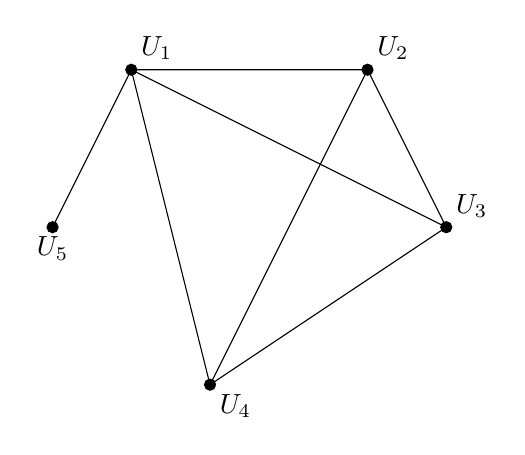
\begin{tikzpicture}
        
        % Points
        \draw[fill=black] (1,1) circle (2pt) node[below] {$U_5$};
        \draw[fill=black] (2,3) circle (2pt) node[above right] {$U_1$};
        \draw[fill=black] (5,3) circle (2pt) node[above right] {$U_2$};
        \draw[fill=black] (6,1) circle (2pt) node[above right] {$U_3$};
        \draw[fill=black] (3,-1) circle (2pt) node[below right] {$U_4$};

        
        % Lines
        \draw (1,1) -- (2,3) -- (5,3) -- (6,1) -- (3, -1) -- (2, 3);
        \draw (6,1) -- (2,3);
        \draw (3, -1) -- (5, 3);
    \end{tikzpicture}
\end{center}
\begin{align*}
    % some math here
    U_1&: U_2, U_3, U_4, U_5 & x_1 = 4 && y = 7 \text{ }(\text{skupno število rokovanj})\\ 
    U_2&: U_1, U_3, U_4      & x_2 = 3 \\
    U_3&: U_2, U_1, U_4      & x_3 = 3 \\
    U_4&: U_1, U_2, U_3      & x_4 = 3 \\
    U_5&: U_1                & x_5 = 1 \\
\end{align*}


\subsubsection{Dokaz}
Naj bodo od $U_1, \dots, U_n$ udeleženci kongresa. Načelo dvojnega preštevanja bomo uporabili na množici urejenih parov $(U_1, U_j)$, za katere se udeleženca $U_i$ in $U_j$ rokojeta. Naj bo $x_i$ število udeležencev s katerimi se je $U_i$ rokoval in $y$ skupno število rokovanj.
\begin{align*}
    % urejeni pari     
\end{align*}
Po eni strani je to število parov enako:
$$
\sum_{i = 1}^{n} x_i
$$
saj je za vsak $U_i$ število izbir enako $x_i$. \\

\noindent
Po drugi strani pa vsako rokovanje poredi natanko dva para:
$$
(U_i, U_j) \text{ in } (U_j, U_i)
$$
skupno število parov je tako $2y$. \\

\noindent
Torej velja:
$$
\sum_{i = 1}^{n} x_i = 2y
$$

$$
4 + 3 + 3 + 3 + 1 = 14
$$
Če pa je vsota $n$ celih števil sodo število lihih sumandov sodo. \\

\noindent
Načelo se navadno uporablja za štetje urejenih parov.


\subsubsection{Izrek}
Naj bosta $A = \{ a_1, \dots, a_m \}$ in $B = \{ b_1, \dots, b_n \}$ množici in naj bo $S \subseteq A \times B$. \\
Naj bo za vse $i = 1, \dots, n$ element $a_i$ prva koordinata $x_i$ parov množice $S$, medtem ko je za vse $j = 1, \dots, n$ element $b_j$ druga koordinata $y_j$ parov množice $S$. Tedaj velja:
$$
|S| = \sum_{i = 1}^{m} x_i = \sum_{j = 1}^{n} y_j
$$


\subsubsection{Zgled}
\begin{align*}
    & A = \{ 1, 2, 3 \} \text{ } B = \{u, v\} \\[1em]
    & A \times B = \{ (1, u), (1, v), (2, u), (2, v), (3, u), (3,v) \} \\[1em]
    & S = \{ (1, u), (1, v), (2, u), (3, v) \}
\end{align*}
\begin{center}

    % dopolni tole

    \begin{tabular}{|c|c|c|}
        \hline
        $(1, u)$ & $(1, v)$ \\  
        \hline
        $(2, u)$ &  \\
        \hline
        & $(3, v)$ \\ 
        \hline
    \end{tabular}    
\end{center}

\subsubsection{Posebni primer}
$x_i$ je konstanta, npr. $x$ in tudi $y_i$ je konstanta, npr. $y$, potem je:
$$
|S| = m \cdot n = n \cdot y
$$


\subsection{Načelo produkta}
Poseben primer načela dvojnega preštevanja je:

\subsubsection{Izrek}
Če sta $A$ in $B$ končni množici, potem velja:
$$
|A \times B| = |A| \cdot |B|
$$

\subsubsection{Dokaz}
Uporabimo prejšnji izrek z množicama $A$ in $B$ kot v izreku, $S = A \times B$ in \\
$x_i = |B|$ za vse $i = 1, \dots, n$. Torej velja:
$$
|A \times B| = |S| = m \cdot |B| = |A| \cdot |B| 
$$
S pmočjo matematične indukcije načelo produkta posplošimo na kartezični produkt \\
poljubnega števila množic $A_1, \dots, A_n$:
$$
|A_1 \times ... \times A_n| = |A_1| \dots |A_n| = \prod_{i = i}^{n} |A_i|
$$


\subsubsection{Zgled}
Koliko je vseh različnih 8-bitnih nizov? Iskani nizi so elementi množice $\{0, 1\}^8$. \\
Vsakega izmed bitov lahko izrazimo na dva načina (0 ali 1) od DOPOLNI po načelu produkta sledi, da DOPOLNI natanko:
$$
|\{0, 1\}|^8 = 2^8 = 256 \text{ } \text{ }\text{ } \text{ (8-bitnih nizov)}
$$

\subsubsection{Zgled}
Študentska restavracija streže 3 vrste predjedi ($P$), 6 glavnih jedi ($G$) in 5 sladic ($S$). Koliko različnih kosil si lahko sestavi študent? Kosilo opišemo kot element množice:
$$
P \times G \times S
$$
različnih kosil pa je potem: $3 \cdot 6 \cdot 5 = 90$.



\subsection{Dirichletovo načelo (načelo golobnjaka)}
Predpostavimo, da je jata golobov priletela v golobnjak. Če je več golobov kot je hišic v golobnjaku, potem bomo vsaj v eni hišici našli vsaj dva goloba.


\subsubsection{Izrek (Dirichletovo načelo)}
Če $n + 1$ ali več predmetov razporedimo v $n$ škatli, potem imamo vsaj v eni škatli vsaj dva predmeta.

\subsubsection{Dokaz}
S protislovjem. Recimo, da je v vsaki škatli največ en predmet.

\begin{center}
    % draw figure of boxes here
\end{center}

\noindent
Potem zaključimo da je vseh predmetov največ $n$, kar je v protislovju s predpostavko, da imamo vsaj $n+1$ predmetov.


\subsubsection{Zgled}
\begin{enumerate}[label=\roman*.]
    \item Vsaki množici z več kot 12 osebami obstajata dve , ki imata rojstni dan v istem mescu. (škatle predstavljajo mesece)
    \item V vsaki množici z več kot 366 osebami obstajata dve, ki imata rojstni dan, na isti dan. (škatle predstavljajo dneve)
    \item Za vsako naravno število $n$ obstaja večkratnik tega števila katerega lahko zapišemo samo s pomočjo cifer 0 in 1. \\[1em]
    \begin{center}
        \begin{tabular}{c|l}
            $n$ &  \\  
            \hline
            1 & 1 \\
            \hline
            2 & 10 \\ 
            \hline
            3 & 111 \\
            \hline
            4 & 100 \\
            \hline
            6 & 1110
        \end{tabular}
    \end{center}
    Naj bo $n$ naravno število. Poglejmo si naslednje zaporedje naravnih števil:
    $$
    1, 11, 111, \dots, \underset{n}{\underbrace{111\ldots 1}}
    $$
    \begin{center}
        \begin{tabular}{r|c}
            $p$ & $p \text{ mod } 6$ \\  
            \hline
            1 & 1 \\
            \hline
            11 & 5 \\ 
            \hline
            111 & 3 \\
            \hline
            1111 & 1 \\
            \hline
            11111 & 5 \\
            \hline
            111111 & 3 \\
        \end{tabular}
    \end{center}
    Če je kakšno izmed njih deljivo z $n$ je problem rešen. V nasprotnem primeru da vsako izmed teh števil pri deljenju z $n$ enega od $n - 1$ možnih ostankov $1, \dots, n - 1$. \\
    Kar je v zaporedju $n$ števil, po \textbf{Dirichletovom načelu} obstajata dve števili v zaporedju, na primer:
    $$
    \underset{k}{\underbrace{11\ldots 1}} \text{ in } \underset{l}{\underbrace{11\ldots 1}}, \text{ } \text{ }\text{ }\text{ } k < l
    $$
    ki data isti ostanek pri deljenju z $n$. Potem pa je njuna razlika:
    $$
    \underset{l - k}{\underbrace{11\ldots 1}}\underset{k}{\underbrace{0 \ldots 0}}
    $$
    deljiva z $n$.
    \item V skupini dveh ali več ljudi lahko vedno najdemo dva, ki imata v tej skupini enako število prijateljev. (predpostavimo, da je relacija prijateljstva simetrična: $x$ je prijatelj z $y$ natanko tedaj, ko je $y$ prijatelj z $x$). Recimo, da skupino sestavlja $n$ ljudi: Razporedimo, ljudi v prostoru glede na to koliko prijateljev imajo.
    \begin{center}
        % make figure here
    \end{center}
    Število prostorov = številu ljudi (in ne moremo na začetku uporabiti Dirichletovega načela), vendar pa opazimo da je vsaj eden od prostorov vedno prazen, če prostor $n - 1$ ni prazen, potem obstaja oseba $x$, ki ima $n - 1$ prijateljev, torej je vsaka oseba prijatelj z osebo $x$ in zato ne obstaja oseba, ki ima 0 prijateljev.
    Torej je $n$ oseb razporejenih v $n-1$ prostorov. Po Dirichletovem načelu obstajata vsaj dve osebi, ki se nahajata v istem prostoru, in imata torej enako število prijateljev.
\end{enumerate}


\subsection{Izrek (posplošeno Dirichletovo načelo)}
Če $m$ predmetov razporedimo v $n$ škatel in velja da je:
$$
m > k \cdot n
$$
potem imamo vsaj v eni škatli vsaj $k + 1$ predmetov. \\[1em]
\fbox{\parbox{1\linewidth}{OPOMBA: \\ Neenakost je najboljša možna. \\ Če je $m = k \cdot n$, lahko vsaka od $n$ škatel vsebuje natanko k objektov.}}

\subsubsection{Zgled}
\begin{enumerate}[label=\roman*.]
    \item 
    \begin{align*}
        \heartsuit \text{ }\text{ }\text{ } 1, \dots, 13 \\
        \diamondsuit \text{ }\text{ }\text{ } 1, \dots, 13 \\
        \clubsuit \text{ }\text{ }\text{ } 1, \dots, 13 \\
        \spadesuit \text{ }\text{ }\text{ } 1, \dots, 13 \\
    \end{align*}
    Najmanj koliko kart moramo izvleči iz standardnega kompleta 52 kart, da bodo med izvlečenimi kartami gotovo štiri karte iste barve (4 $\heartsuit$ ali 4 $\diamondsuit$ ali 4 $\clubsuit$ ali 4 $\spadesuit$)?
    \begin{align*}
        % draw figure here
        \text{predmeti = karte} \text{ }\text{ }\text{ } & k + 1 = 4 \\
        \text{škatle = barve} \text{ }\text{ }\text{ } & k = 3 \\
    \end{align*}
    Predpostavimo da imamo 4 škatle, vsako rezerviramo z posamezno barvo. Ko karto izvlečemo, jo damo v pripadajočo škatlo. Iz posplošenega Drirchletovega načela vidimo, da je dovolj izvleči:
    $$
    13 \text{ }\text{ }\text{ } ( = 3 \cdot 4 + 1)
    $$
    kart, da bodo med izvlečenimi kartami gotovo štiri iste barve.
    \item V množici šestih oseb vedno obstajajo tri osebe ki se poznajo med sabo, ali pa obstajajo tri osebe, ki se ne poznajo med sabo.
    \begin{center}
        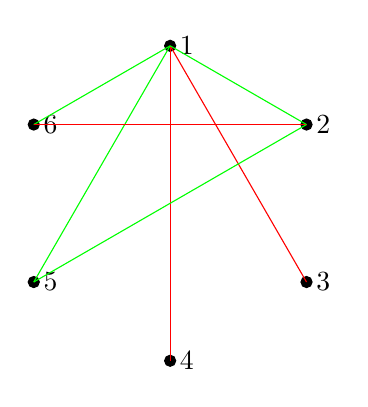
\begin{tikzpicture}
        
            % Define the coordinates for the vertices of a regular hexagon
            \coordinate (1) at (90:2); % 1
            \coordinate (2) at (30:2); % 2
            \coordinate (3) at (-30:2); % 3
            \coordinate (4) at (-90:2); % 4
            \coordinate (5) at (-150:2); % 5
            \coordinate (6) at (150:2); % 6
    
            % Draw the vertices and label them
            \foreach \i/\label in {
                1/1,
                2/2,
                3/3,
                4/4,
                5/5,
                6/6
            } {
                \draw[fill=black] (\i) circle (2pt) node[right] {\label};
            }
    
            \draw[red] (90:2) -- (-90:2);
            \draw[red] (90:2) -- (-30:2);
            \draw[green] (90:2) -- (30:2);
            \draw[green] (90:2) -- (-150:2);
            \draw[green] (90:2) -- (150:2);

            \draw[red] (30:2) -- (150:2);
            \draw[green] (30:2) -- (-150:2);
        \end{tikzpicture}
    \end{center}
    
    Naj bo $a$ poljubno izbrana oseba iz množice. \\
    Razdelimo naslednjih 5 oseb v dva prostora.
    \begin{center}
        
    \end{center}
    Ker je $5 > 2 \cdot 2$, po Dirichletovem načelu obstaja en prostor z vsaj 3 osebami.
    \begin{center}
        % figure again
    \end{center}
    Predpostavimo najprej, da so v prvem prostoru osebe $b, c, d$. Če se kakšni dve izmed teh oseb poznata med seboj, na primer $b$ in $c$ potem je $\{a, b, c\}$ podmnožica teh oseb ki se med seboj poznajo. V nasprotnem primeru pa se nobeni dve osebi iz podmnožice $\{b, c, d\}$ ne poznata. Primer, ko se ti osebi nahajajo v drugem prostoru, obravnavamo podobno.
\end{enumerate}
